\documentclass[paper=a4,UTF8,fontsize=11pt]{scrartcl} % A4 paper and 11pt font size
\usepackage[noend]{algpseudocode}
\usepackage{ctex}
\usepackage[T1]{fontenc} % Use 8-bit encoding that has 256 glyphs
\usepackage{fourier} % Use the Adobe Utopia font for the document - comment this line to return to the LaTeX default
\usepackage[english]{babel} % English language/hyphenation
\usepackage{amsmath,amsfonts,amsthm} % Math packages
\usepackage[english]{babel}
\usepackage[utf8]{inputenc}
\usepackage{indentfirst}
\usepackage{algorithm}
\usepackage{lipsum} % Used for inserting dummy 'Lorem ipsum' text into the template
\usepackage{float}
\usepackage{sectsty} % Allows customizing section commands
\allsectionsfont{\centering \normalfont\scshape} % Make all sections centered, the default font and smaıll caps
\usepackage{graphicx}
\usepackage{fancyhdr} % Custom headers and footers
\pagestyle{fancyplain} % Makes all pages in the document conform to the custom headers and footers
\fancyhead{} % No page header - if you want one, create it in the same way as the footers below
\fancyfoot[L]{} % Empty left footer
\fancyfoot[C]{\thepage} % Empty center footer
\fancyfoot[R]{} % Page numbering for right footer
\renewcommand{\headrulewidth}{0pt} % Remove header underlines
\renewcommand{\footrulewidth}{0pt} % Remove footer underlines
\setlength{\headheight}{13.6pt} % Customize the height of the header
\usepackage[noend]{algpseudocode}
\numberwithin{equation}{section} % Number equations within sections (i.e. 1.1, 1.2, 2.1, 2.2 instead of 1, 2, 3, 4)
\numberwithin{figure}{section} % Number figures within sections (i.e. 1.1, 1.2, 2.1, 2.2 instead of 1, 2, 3, 4)
\numberwithin{table}{section} % Number tables within sections (i.e. 1.1, 1.2, 2.1, 2.2 instead of 1, 2, 3, 4)
\usepackage{color}
\setlength\parindent{0.3pt} % Removes all indentation from paragraphs - comment this line for an assignment with lots of text
\usepackage{graphicx}
\usepackage{xcolor}
\usepackage{listings}
\definecolor{mygreen}{rgb}{0,0.6,0}
\definecolor{mygray}{rgb}{0.5,0.5,0.5}
\definecolor{mymauve}{rgb}{0.58,0,0.82}

\lstset{ 
  language=C++,
  backgroundcolor=\color{white},   % choose the background color
  basicstyle=\footnotesize,        % size of fonts used for the code
  breaklines=true,                 % automatic line breaking only at whitespace
  captionpos=b,                    % sets the caption-position to bottom
  commentstyle=\color{mygreen},    % comment style
  escapeinside={\%*}{*)},          % if you want to add LaTeX within your code
  keywordstyle=\color{blue},       % keyword style
  stringstyle=\color{mymauve},     % string literal style
}
% \lstset{language=C++,
%                 basicstyle=\ttfamily,
%                 keywordstyle=\color{blue}\ttfamily,
%                 stringstyle=\color{red}\ttfamily,
%                 commentstyle=\color{green}\ttfamily,
%                 morecomment=[l][\color{magenta}]{\#}
% }



%----------------------------------------------------------------------------------------
%	TITLE SECTION
%----------------------------------------------------------------------------------------

\newcommand{\horrule}[1]{\rule{\linewidth}{#1}} % Create horizontal rule command with 1 argument of height
\title{
\normalfont \normalsize
\textsc{Shanghai Jiao Tong University} \\ [25pt] % Your university, school and/or department name(s)
\horrule{0.5pt} \\[0.4cm] % Thin top horizontal rule
\huge 内部算法排序 \\ % The assignment title
\horrule{2pt} \\[0.5cm] % Thick bottom horizontal rule
}

\author{\\ \kaishu 吕艺\\ \normalsize 517021910745} % Your name

\date{\normalsize\today} % Today's date or a custom date

\begin{document}

\maketitle % Print the title
\kaishu
\section{需求分析}

1.本演示文件的主要需求为判断各种排序方法的比较次数和移动次数,涉及到的排序方法分别为冒泡排序,直接插入排序,简单选择排序,快速排序,
希尔排序和堆排序。首先先生成随机数num,代表随机数个数。根据每组随机数个数不超过100个的要求,本演示文件中选择了每组随机数的个数在100~1000个。
根据随机数的组数不少于5的条件,本演示文件中选择的随机数组数为8组。
\vspace{0.5cm}

2.演示文件无需用户输入,文件运行结束后即在计算机终端上打印运算结果,显示在屏幕上。
\vspace{0.5cm}
\newpage

3.程序执行的命令包括:
\begin{enumerate}
    \item 根据系统时间生成随机数个数。
    \item 根据系统时间和事先生成的随机数个数生成随机数数组
    \item 利用上述六种排序方式对随机数数组进行从小到大的排序
    \item 将每种排序方式的比较次数和移动次数打印在屏幕上
\end{enumerate}

\vspace{0.8cm}

4.测试数据

本演示文件中用到的测试数据均为随机生成的数组
\vspace{0.8cm}

\section{概要设计}

本演示文件中涉及到排序方式多样,例如插入排序中的直接插入排序和希尔排序,选择排序中的直接选择排序,堆排序,
交换排序中的冒泡排序和快速排序。

1.哈夫曼类 $hfTree$

数据对象: Node *elem;\ \ \ \ \ \ \ \ int length;

私有类:   struct Node \{

    \qquad \qquad \ \  Type data;

    \qquad \qquad \ \ int weight; \}; 

    \qquad \qquad \ \ struct hfCode \{
        
    \qquad \qquad \ \ Type data;

    \qquad \qquad \ \ string Code;\};

基本操作:hfTree(const Type *x, const int *w, int size);

\qquad \qquad \quad \ \ \ 操作条件: 哈夫曼树还未被初始化

\qquad \qquad \quad \ \ \ 操作结果: 利用传入参数初始化哈夫曼树

\qquad \qquad \quad \ \ \ void getCode(hfCode result[]) const;

\qquad \qquad \quad \ \ \ 初始条件: 哈夫曼树已被建好

\qquad \qquad \quad \ \ \ 操作结果: 形成含有编码的$Node$类型的数组

\qquad \qquad \quad \ \ \ hfTree(const hfTree \& myTree);

\qquad \qquad \quad \ \ \ 初始条件:哈夫曼树已经被初始化

\qquad \qquad \quad \ \ \ 操作条件: 将传入的树 $MyTree$ 的各个数据对象复制给该树

\qquad \qquad \quad \ \ \  ~hfTree() { delete[] elem; }

\qquad \qquad \quad \ \ \  操作条件: 哈夫曼树存在

\qquad \qquad \quad \ \ \ 操作结果: 释放哈夫曼树中$elem$所占的内存

\qquad \qquad \quad \ \ \ Node *GetElem() const { return elem; }

\qquad \qquad \quad \ \ \ 操作条件: 哈夫曼树存在

\qquad \qquad \quad \ \ \ 操作结果:返回指针$elem$

\qquad \qquad \quad \ \ \ int GetLength() const { return length; }

\qquad \qquad \quad \ \ \ 操作条件: 哈夫曼树存在

\qquad \qquad \quad \ \ \ 操作结果: 返回哈夫曼叶子结点的个数
\vspace{0.3cm}

2.本程序包括两个模块:

1)  int main() \{

    \ \  while(Command != 'E')\{

        \ \  Process Command;

        \ \  input Command;\} \}
       
2)  哈夫曼树单元模块--实现哈夫曼树的构建和编码

\section{详细设计}
1)哈夫曼树单元模块
\lstinputlisting{Part.h}

2)主函数模块
\lstinputlisting{main.cpp}

3)函数指针模块
\lstinputlisting{FuncPointer.h}
\vspace{0.3cm}
\section{调试分析}
1.一开始本演示文件对于哈夫曼树仅设计了含有形参的初始化函数,因此哈夫曼树仅能在参数给定后被初始化(在本题中只能在初始化函数作用域中被使用,函数调用结束后就会被析构),
这导致初始化后必须保存参数,并在每次执行其他操作时新建一棵树,大大降低的时间效率,提高了复杂度。为了解决这一问题,本演示文件中重载了初始化函数,并在主函数内定义了一棵默认哈弗曼树。
调用初始化函数后利用重载的拷贝构造函数保存下初始化的树,在主函数作用域中都可用。

2.一开始由于对输入情况考虑的欠缺,本演示文件一开始把哈弗曼树的节点值设为了字符型。为了加强类的泛化能力,本演示文件采用模板类以及模板函数,从而使文件的适用范围更广。

3.算法的复杂度分析

1)时间复杂度
由于采用数组的形式存储哈弗曼树,各种操作的算法复杂度比较合理。
initial 函数和Decoding函数的时间复杂度是$O(n^{2})$, 函数Codeprinting和函数Treeprinting的时间复杂度均为$O(n)$,而Encoding函数的时间复杂度是$M(max\{O(m^{2}),O(n^{2}\})$
(设文件读入规模为m,哈弗曼树叶节点个数为n)。

initial函数在调用初始化函数时利用双层循环遍历进行树的合并,而Decoding函数中也利用双层循环读入文件的编码并寻找到对应字符的编码输出到文件中,因此这两个函数的时间复杂度为$O(n^{2})$。
Encoding函数从文件中读入m个字符并在n个字符中找到对应字符的编码输出,所以时间复杂度为$M(max\{O(m^{2}),O(n^{2}\})$。
Codeprinting函数和Treeprinting函数的时间复杂度主要决定于编码长度和哈弗曼树节点个数,因此时间复杂度与元素个数成正比,因此时间复杂度为$O(n)$。

2)空间复杂度

哈弗曼树模块的空间复杂度与叶节点的个数成正比,即$O(n)$。
主函数模块的复杂度取决于定义主函数作用域中的哈弗曼树,故空间复杂度也为$O(n)$。
\vspace{0.5cm}
\section{用户手册}
1.本程序以Jetbrains Clion 2018.2.5, 采用C++ 11 标准,程序以项目方式组织(project),如图1所示:
\begin{figure}[h]
    \centering
    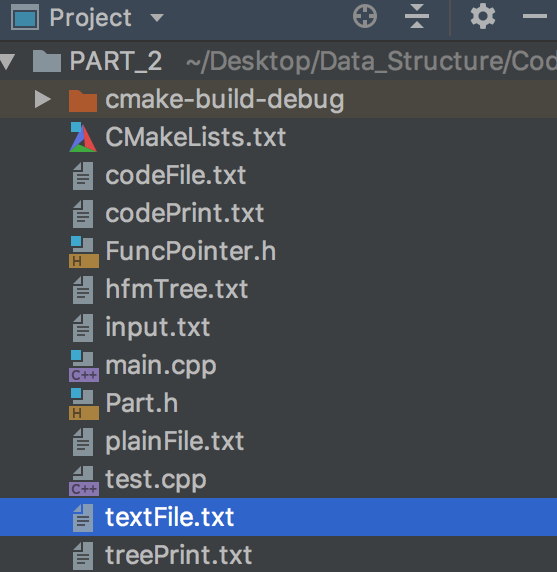
\includegraphics[width=0.6\textwidth]{project.png}
\end{figure}
\newpage
2.依次点击菜单"Run"->build,再点击"Run",显示文本方式的用户界面,如图 2 所示:
\begin{figure}[h]
    \centering
    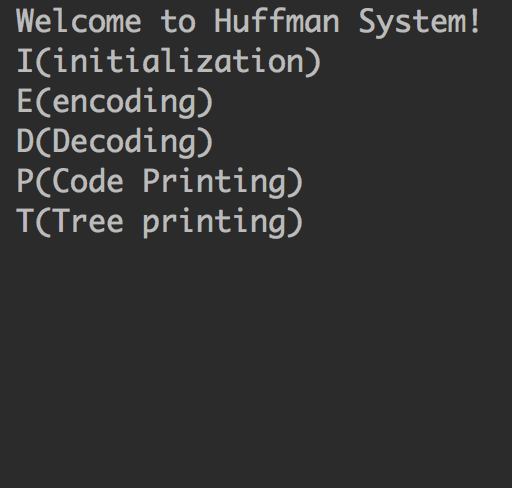
\includegraphics[width=0.6\textwidth]{interface.png}
\end{figure}

3.键入操作命令符后按“回车键”,程序就执行相应命令(用户需在初始化时输入对应参数)。有效的命令
符为 I,E,D,P,T 或 Q。若输入的命令符无效,提示并要求重新输入命令符。

\section{测试结果}
执行命令'I'后:输入测试数据2中的参数和权重,建立哈弗曼树
执行命令'E'后:在文件PlainFile中输入"THIS PROGRAM IS MY FAVORITE",将编码存储到codeFile中
执行命令'D'后:新建文件textFile,将文件codeFile中的编码翻译成"THIS PROGRAM IS MY FAVORITE"
执行命令'P'后:在屏幕上打印codeFile中的编码,并保存到codePrint中
执行命令'T'后:将已建好的哈弗曼树以凹入表的形式存储到treePrint文件中

\section{附录}

源程序文件名清单

main.cpp                //主函数

Part.h                  //哈夫曼树单元模块

FuncPointer.h           //函数指针模块



\end{document}



